% !TeX spellcheck = en_US
\documentclass[a4paper]{scrartcl}

\usepackage[utf8]{inputenc}
\usepackage[english]{babel}
\usepackage[T1]{fontenc}
\usepackage{lmodern}
\usepackage{amsmath}
\usepackage{amssymb}
\usepackage{pdflscape}
\usepackage{geometry}
\usepackage{xcolor}
\usepackage{graphicx}
\usepackage{todonotes}
\setlength{\parindent}{0pt}

\usepackage{biblatex}
\addbibresource{references.bib}


%\geometry{a4paper, top=25mm, left=30mm, right=20mm, bottom=30mm,
%headsep=10mm, footskip=12mm}

\newcommand{\itab}[1]{\hspace{0em}\rlap{#1}}
\newcommand{\tab}[1]{\hspace{.2\textwidth}\rlap{#1}}


\title{Proposal for the Master's Thesis\\Grammar-based Recompression with Adjacent Digrams}
\author{Matthias Dürksen}
\date{\today}
 

\begin{document}
\maketitle

\section{Motivation}\label{sec:motivation}

Nowadays, there is more and more data, some of it is stored in graphs. The graphs often become very large and therefore require a lot of memory. To solve this problem, you can compress the graph in order to reduce the memory requirements. In this thesis a grammar-based graph compression is used. An approach to grammer-based compression for graphs was already invented by me in a previous work~\cite{mattdk}.

This concept~\cite{mattdk} has already been extended in several bachelor theses. There is a recompression for already compressed graphs~\cite{werneke} and also an efficient coding~\cite{georgi}. For reasons of complexity, a compression options, the so-called adjacency digrams, was not supported in the further work, which significantly limits the compression efficiency. 
The overall aim of this work is to support adjacency digrams also in recompression and coding.



\section{Fundamentals}


Graph compression supports graphs with nodes and edge labels. With my approach, the graph is first converted. The result of the conversion is a graph with only node labels and no edge labels, which facilitates compression. 

After the conversion comes the transformation. Hereby, patterns (which are called digrams) are searched and the most frequent pattern/digram is replaced by a nonterminal symbol.
We distinguish between two types of digrams, the basic and the adjacency digrams.
A basic digram (Fig.~\ref{fig:basicDigram}) consists of two adjacent nodes and the edge that connects these nodes. Thus, two adjacent nodes and the incident edge can be replaced by one nonterminal symbol.
\begin{figure}[h]
	\centering
	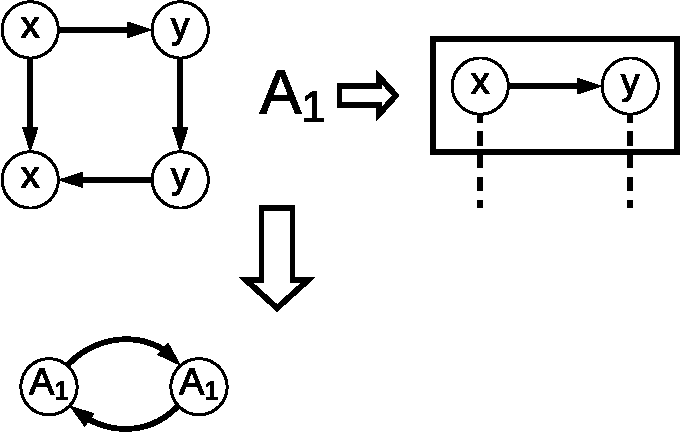
\includegraphics[width=0.4\textwidth]{img/basicDigram}
	\caption{Application of a replacement of a basic digam}
	\label{fig:basicDigram}
\end{figure}

The adjacency digram (Fig.~\ref{fig:adjazenzDigram}) is formed by two nodes which both have a common adjacency node x. Thus, the adjacency digram contains the two nodes and the two edges that are incident to the node x. This digram can be replaced by a nonterminal and an edge from the nonterminal to the node x.
Thus, the possibilities of replacement by the adjacency digram are significantly increased.


\begin{figure}[h]
	\centering
	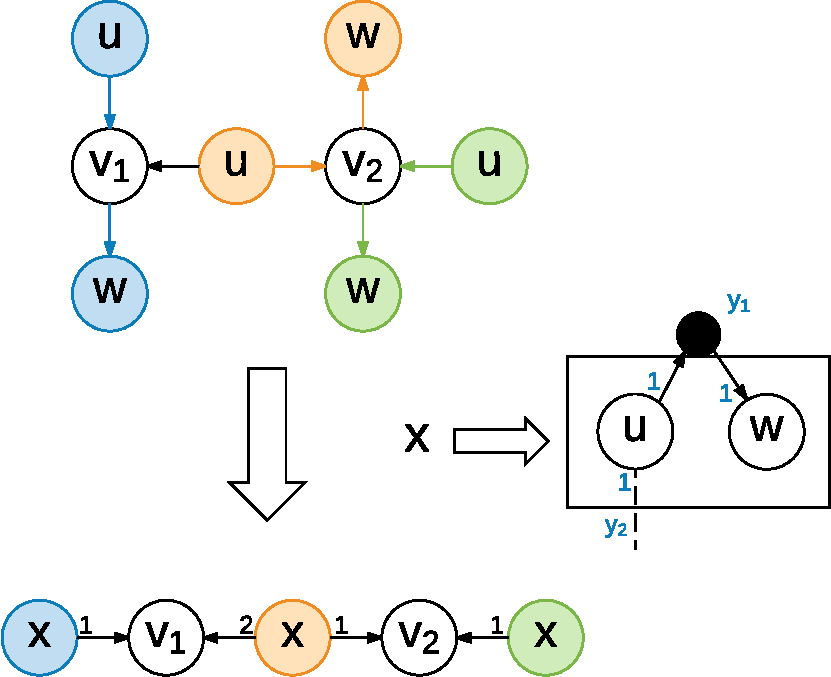
\includegraphics[width=0.5\textwidth]{img/adjazenzDigram}
	\caption{Application of a replacement of an adjacency digam}
	\label{fig:adjazenzDigram}
\end{figure}

After the search for the most frequent digram, all non-overlapping occurrences are replaced by the nonterminal. Then, the search for the most frequent digram and the replacement of the occurrences is continued until there are no more digrams which occur frequently enough.



\section{This Thesis}

These compressed graphs and the corresponding grammar rules can be coded on the basis of Georgi's work~\cite{georgi} and thus save the graph in a memory efficient way. However, this coding is only designed for graphs where there have been no replacements based on the adjacency digrams. Therefore it is part of the work to extend this coding to support graphs where adjacency digrams have been replaced.

Furthermore, the works of Frerk~\cite{pfrerk} and Werneke~\cite{werneke} have developed an extension for the recompression of graphs. This method can be used if, for example, two subgraphs were compressed individually and these graphs are compressed together. This method combines the two graphs and checks whether the grammar rules can be chosen more efficiently in the combination of the two graphs than to combine the previous rules. This method can also be used if an existing graph has been modified and thus has new nodes or old nodes have been removed. Thus, it is checked again whether there is now an efficient compression.

Frerk's approach is based on the graph model and Werneke's methods work on memory level, so that Georgi's coding is considered here. However, it also only supports the basic digrams.
Therefore, the procedure of~\cite{werneke} is to be extended so that also here the adjacency digrams are supported.

However, Frerk has already discussed and supported the treatment in his work, so it is also necessary to examine which parts of the Frerk procedure can be applied to the other procedure. (Need for clarification with the supervisor)


\pagebreak
\printbibliography







\end{document}